\section{Merging data}
\label{sec:join}

In many cases, we need to combine data from different sources or data files.
For example, we might have election poll results in one file and socio-economic data per area in another.
To test whether we can explain variance in poll results from factors such as education level,
we would need to combine the poll results with the economic data.
This process is often called merging or joining data.

\subsection{Equal units of analysis}

%\pyrex[caption=Private and Pulic Capital data (source: Piketty 2014)]{ch_data_wrangling/piketty}

\begin{ccsexample}
  \doublecodex{ch_data_wrangling/piketty_1}
  \codexoutputtable{ch_data_wrangling/piketty_1.r}
  \doublecodex{ch_data_wrangling/piketty_2}
  \codexoutputtable{ch_data_wrangling/piketty_2.r}
\caption{Private and Pulic Capital data (source: Piketty 2014)}\label{ex:piketty}
\end{ccsexample}


The easiest joins are when both data sets have the same unit of analysis,
i.e. the rows represent the same units.
For example, consider the data on public and private capital ownership published by
\cite{piketty} alongside his landmark book \emph{Capital in the 21st Century}.
As shown in \refex{piketty}, he released separate files for public and private capital ownership.
If we would want to analyse the relationship between these (for example to recreate Figure 3.6 on page 128 of that book),
we first need to combine them into a single data frame.

To combine these data frames, we use the \pkg{pandas} data frame method \fn{merge} in Python or the \pkg{dplyr} method \fn{full\_join} in R.
Both methods join the data frames on one or more \emph{key} columns.
The key column(s) identify the units in both data frames, so in this case the \emph{Year} column.
Often, the key column is some sort of identifier, like a respondent or location ID.
The resulting data frame will contain the shared key column(s), and all other columns from both joined data frames.

In both Python and R, all columns that occur in both data frames are by default assumed to be the key columns.
In many cases, this is the desired behaviour as both data frame may contain e.g. a \emph{Year} or \emph{RepondentID} column.
Sometimes, however, this is not the case.
Possibly, the key column is called differently in both data frames, e.g. \emph{respID} in one and \emph{Respondent} in the other. 
It is also possible that the two frames contain columns with the same name,
but which contain actual data that should not be used as key.
For example, in the Piketty data shown above the key column is called \emph{Year} in both frames,
but they also share the columns for the countries which are data columns.

In these cases, it is possible to explicitly specify which columns to join on (using the \verb+on=+ (Python) / \verb+by=+ argument).
However, we would generally recommend preprocessing the data first and select and/or rename columns such that the only shared columns are the key columns.
The reason for that is that if columns in different data frames mean the same thing (i.e. \emph{respID} and \emph{Respondent}), they should generally have the same name to avoid confusion.
In the case of `accidentally' shared column names, such as the country names in the current example,
it is also better to rename them so it is obvious which is which in the resulting data set:
if shared columns are not used in the join, by default they get `.x' and `.y' (R) or `\_x' and `\_y' (Python) OA appended to their name, which is not very meaningful.
Even if the key column is the only shared column, however, it can still be good to explicitly select that column to make it clear to the reader (or for yourself in the future) what is happening. 

\begin{ccsexample}
\doublecodex{ch_data_wrangling/capital_1}
\codexoutputtable{ch_data_wrangling/capital_1.r}
\doublecodex{ch_data_wrangling/capital_2}
\doubleoutput{ch_data_wrangling/capital_2}
\caption{Merging private and public data for France}\label{ex:merge}
\end{ccsexample}


%\pyrex[caption=Merging private and public data for France]{ch_data_wrangling/capital}

This is shown in \refex{merge}.
The first two lines select only the \emph{Year} and \emph{France} columns, and rename the \emph{France} column to indicate whether it is the private or public data.
Lines 3 and 5 do the actual join, with and without the explicit selection of key column, respectively.
This is then used to compute the correlation between private and public capital, 
which shows that there is a weak but (just) significant negative correlation ($\rho=-.32, p=.04$)%
\footnote{Of course, the fact that this is time series data means that the independence assumption of regular correlation is violated badly, so this should be interpreted as a descriptive statistic, e.g. in the years with high private capital there is low public capital and the other way around}.

\note{Next to \fn{merge}, pandas dataframes also have a method called \fn{join}. It is a simplified version for joining on indices (i.e., the row labels). If you have two data frames in which corresponding rows have the same row number, you can simply write \texttt{df1.join(df2}. In short: both methods do the same, but merge provides more options, and join is easier if you want to join on the indices.}



\subsection{Inner and Outer joins}

In the example above, both data sets had exactly one entry for each unit (year), making it the most straightforward case.
If either (or both) of the data sets are missing units, however, you need to specify how to deal with this.

\reftab{joins} list the 4 possible ways of joining, keeping all rows (\emph{outer join}), only rows present in both (\emph{inner join}), or all rows from one of the sets and matching rows from the other (\emph{left} or \emph{right join}). Left and right here literally refer to the order in which you type the dataframe names. Figure~\ref{fig:joinvenn} and Table~\ref{tab:joins} give an overview. 
In all cases except inner joins, this can create units where information from one of the data sets is missing.
This will be lead to missing values (|NA|/|NaN|) being inserted in the columns of the data sets with missing units.

%

\def\venna{(0,0) circle (0.8cm)}
\def\vennb{(1cm,0) circle (0.8cm)}

\begin{tabularx}{\textwidth}{cccc}
  Left join & Right join & Inner Join  & Outer Join\\
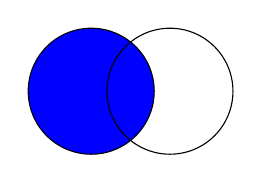
\begin{tikzpicture}
  \fill[blue] \venna;
  \draw\venna;
  \draw\vennb;
\end{tikzpicture}
&
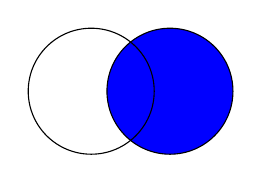
\begin{tikzpicture}
  \fill[blue] \vennb{};
  \draw\venna;
  \draw\vennb;
\end{tikzpicture}
&
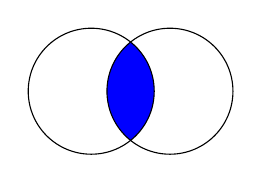
\begin{tikzpicture}
  \begin{scope}
    \clip\venna;
    \fill[blue] \vennb;
    \end{scope}
  \draw\venna;
  \draw\vennb;
\end{tikzpicture}
&
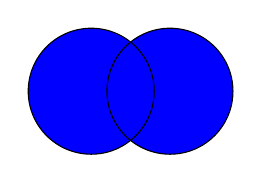
\begin{tikzpicture}
  \fill[blue] \venna;
  \fill[blue] \vennb;
  \draw\venna;
  \draw\vennb;
\end{tikzpicture}
\\
\end{tabularx}

\begin{figure}
    \centering
    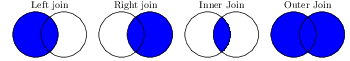
\includegraphics{figures/ch07_figjoins}
    \caption{The solid area indicades whether the cases in the resulting datasets need to appear in one, both, or any of the datasets.}
    \label{fig:joinvenn}
\end{figure}

\SaveVerb{py_full}|d1.merge(d2, how='outer')|
\SaveVerb{py_inner}|d1.merge(d2, how='inner')|
\SaveVerb{py_left}|d1.merge(d2, how='left')|
\SaveVerb{py_right}|d1.merge(d2, how='right')|
\SaveVerb{r_full}|full_join(d1,d2)|
\SaveVerb{r_inner}|inner_join(d1,d2)|
\SaveVerb{r_left}|left_join(d1,d2)|
\SaveVerb{r_right}|right_join(d1,d2)|


\begin{table}
  \caption{Different types of joins between datasets d1 and d2\label{tab:joins}}{%
  \begin{tabularx}{\linewidth}{lXll}
    \toprule
    Type &  Description  & R & Python \\
    \midrule
    Outer &  All units from both sets & \UseVerb{r_full} & \UseVerb{py_full} \\
    Inner & Only units that are in both sets & \UseVerb{r_inner} & \UseVerb{py_inner} \\
    Left & All units from left-hand set & \UseVerb{r_left} & \UseVerb{py_left} \\
    Right & All units from right-hand set & \UseVerb{r_right} & \UseVerb{py_right} \\  
    \bottomrule
  \end{tabularx}}{}
\end{table}


In most cases, you will either use inner join or left join.
Inner join is useful when information should be complete,
or where you are only interested in units with information in both data sets.
In general, when joining sets with the same units, it is smart to check the number of rows before and after the operation.
If it decreases, this shows that there are units where information is missing in either set.
If it increases, it shows that apparently the sets are not at the same level of analysis,
or there are duplicate units in the data.
In either case, an unexpected change in the number of rows is a good indicator that something is wrong.

Left joins are useful when you are adding extra information to a `primary' data set.
For example, you might have your main survey results in a data set,
to which you want to add metadata or extra information about your respondents.
If this data is not available for all respondents, you can use a left join to add the information
where it is available, and simply leave the other respondents with missing values.


A similar use case is when you have a list of news items, and a separate list of items that were coded
or found with some search term. Using a left join will let you keep all news items, and add the coding where it is available.
Especially if items that had zero hits of a search term are excluded from the search results,
you might use a left join followed by a calculation to replace missing values by zeroes to indicate that the counts for
items aren't actually missing, but were zero. 

Of course, you could also use a right join to achieve the same effect.
It is more natural, however, to work from your primary data set and add the secondary data,
so you will generally use left joins rather than right joins.

Outer (or full) joins can be useful when you are adding information from e.g. multiple survey waves,
and you want to include any respondent that answered any of the waves.
Of course, you will have to carefully think about how to deal with the resulting missing values in the substantive analysis. 

\subsection{Nested data}

The sections above discuss merging two data sets at the same level of analysis,
i.e. with rows representing the same units (repondents, items, years) in both sets.
It is also possible, however, to join a more aggregate (high level) set with a more detailed data set.
For example, you might have respondents that are part of a school or organizational unit.
It can be desirable to join the respondent level information with the school level information,
for example to then explore differences between schools or do multilevel modelling.

For this use the same commands as for equal joins.
In the resulting merged data set, information from the group level will be duplicated for all individuals in that group.

For example, take the two data sets shown in \refex{primary}.
The \texttt{results} data set shows how many votes each US 2016 presidential primary candidate received in each county:
Bernie Sanders got 544 votes in Autauga County in the US state of Alabama, which was 18.2\% of all votes cast in the
Democratic primary.
Conversely, the \texttt{counties} data set shows a large number of facts about these counties,
such as population, change in population, gender and education distribution, etc. 

\pyrex[caption={2016 Primary results and county-level metadata. Note that to avoid duplicate output, we display the counties data in the Python example and the results data in the R example.}]{ch_data_wrangling/primary}

Suppose we hypothesize that Hillary would do relatively well in areas with more black voters.
We would then need to combine the county level data about ethnic composition with the country $\times$ candidate
level data on vote outcomes.

This is achieved in \refex{nested} in two steps.
First, both data sets are cleaned to only contain the relevant data:
for the \texttt{results} data set only the Democrat rows are kept, and only the \emph{fips} (county code), \emph{candidate}, \emph{votes}, and \emph{fraction} columns.
For the \texttt{counties} data set, all rows are kept but only the \emph{county code}, \emph{name}, and \emph{Race\_white\_pct} columns are kept.

\pyrex[caption=Joining data at the result and the county level]{ch_data_wrangling/nested}

In the next step, both sets are joined using an inner join from the results data set.
Note that we could also have used a left join here, but with an inner join it will be immediately
obvious if county level data is missing, as the number of rows will then decrease.
In fact, in this case the number of rows does decrease, because some results do not have corresponding county data.
As a puzzle, can you use the dataset filtering commands discussed above to find out which results these are?

Note also that the county level data contains units that are not used, particularly the national and state level statistics.
These, and the results that do not correspond to counties, are automatically filtered out by using an inner join.

Finally, we can create a scatter plot or correlation analysis of the relation between ethnic composition and electoral success (see how to create the scatter plot in section \refsec{visualization}).
In this case, it turns out that Hillary Clinton did indeed do much better in counties with a high percentage of black residents.
Note that we cannot take this to mean there is a direct causal relation, there could be any number of underlying factors, including the date of the election which is very important in primary races.
Statistically, since observations within a state are not independent, we should really control for the state-level vote here.
For example, we could use a partial correlation, but we would still be violating the independence assumption of the errors,
so it would be better to take a more sophisticated (e.g. multilevel) modeling approach. This, however, is well beyond the scope
of this chapter. 

% TODO! By selecting only one candidate, the levels actually are equal :(
